% =============================================================================
\chapter{Probabilistic representation of Bell inequalities violation}
\label{cha:bell-ineq}
% =============================================================================

In this final chapter we will diverge from the central topic of this thesis~--- the Wigner representation~--- and briefly discuss other quasiprobability representations.
In particular we will be interested in their ability to model such an inherent property of quantum systems as an entanglement~\cite{Einstein1935}, and a consequent violation of Bell inequalities~\cite{Bell1964}.
The possibility of this is often discarded because of the famous Feynman's lecture~\cite{Feynman1982}, where he posed a question \textit{``Can quantum systems be probabilistically simulated by a classical computer?''}, and his final answer was \textit{``If ... there's no hocus-pocus, the answer is certainly, No!''}.
His argument was based on the assertion that Bell violations cannot be modeled probabilistically~\cite{Bell1964}.

However, it turns out that positive phase-space distributions of quantum optics~\cite{Husimi1940,Drummond1980,Hillery1984,Gardiner2004} are capable of such simulations, owing to extended range of the functions of phase-space variables corresponding to physical observables as compared to those considered by Bell.
Namely, these functions can have a continuous range of values extending beyond the set of discrete expected values for the physical quantity, and, furthermore, their values can be complex~\cite{Reid1986}.
The expectations of such observables correspond to physical quantities only when integrated with the phase-space distribution as a weight.
This method of simulation is analogous to the weak measurement strategy, or \abbrev{povm} (positive operator valued measure)~\cite{Aharonov1988}, which has been experimentally demonstrated recently~\cite{Goggin2011}.

% acknowledgement
The idea of computationally demonstrating the violation of Bell inequalities using quasiprobability representations belongs to M.~D.~Reid.


% =============================================================================
\section{Cooperative states}
% =============================================================================

A Bell inequality sets a limit on observable correlations in a physical system that obeys a local hidden variable theory (\abbrev{lhv})~\cite{Bell1964,Clauser1969}.
This is a classical theory where the results of the measurements are functions of local detector settings and a hidden parameter $\lambda$.
Thus, values measured by two spatially separated observers, $A$ and $B$ (for Alice and Bob, as they are usually denoted), can be expressed as $A(a, \lambda)$ and $B(b, \lambda)$, where $a$ and $b$ are Alice's and Bob's detector settings.
Possible correlations are defined probabilistically as
\begin{eqn}
\label{eqn:bell-ineq:cooperative:lhv}
    C(A,B)
    = \int_{\Lambda} A(a, \lambda) B(b, \lambda) P(\lambda) \upd\lambda.
\end{eqn}
Experimental values $A$ and $B$ are usually encoded as either $1$ or $-1$ in a binary experiment.
The Bell theorem derives inequalities that any such correlations in a \abbrev{lhv} theory must satisfy.
Quantum mechanics violates these inequalities, thus ruling out \abbrev{lhv} theories.


% =============================================================================
\subsection{Quantum state}
% =============================================================================

In this section we will consider Bell violations in cooperative states with $N$ photon pairs, similar to those demonstrated experimentally by Clauser~\cite{Clauser1969}, Aspect \textit{et~al}~\cite{Aspect1982}, and Zeilinger \textit{et~al}~\cite{Weihs1998}.
The quantum state in question is
\begin{eqn}
\label{eqn:bell-ineq:cooperative:state}
    \vert N \rangle
    = \frac{%
        \left(
            \hat{a}_{1+}^{\dagger} \hat{a}_{2+}^{\dagger}
            + \hat{a}_{1-}^{\dagger} \hat{a}_{2-}^{\dagger}
        \right)^{N} \vert 0 \rangle%
        }{N! \left( N+1 \right)^{1/2}},
\end{eqn}
where $N$ is the number of photon pairs, indices $1$ and $2$ denote the propagation direction, and $+$ and $-$ stand for the polarization direction.
These states are generated in certain types of optical parametric down-conversion experiments, and it has proved difficult to obtain a direct, loophole free violation of a Bell inequality, owing to detector inefficiencies~\cite{Cabello2007,Larsson1998,Larsson2001}.
However, these issues are not significant for the simulations in this thesis since we are considering an ideal experiment.

We define the intensity correlations to be~\cite{Drummond1983}
\begin{eqn}
\label{eqn:bell-ineq:cooperative:G}
    G^{IJ}(\gamma,N)
    = \langle N \vert
        \hat{A}^{I}(1,\hat{\avec}_{1})
        \hat{A}^{J}(\gamma,\hat{\avec}_{2})
        \vert N \rangle,
\end{eqn}
where $\gamma$ is a linear combination parameter related to the polarizer angle, and auxiliary functions are introduced so that:
\begin{eqn}
    \hat{A}^{J}(\gamma,\hat{\avec}_{k})
    ={} & \left(
            \sqrt{\gamma} \hat{a}_{k-}^{\dagger}
            + \sqrt{1-\gamma} \hat{a}_{k+}^{\dagger}
        \right)^{J}
        \left(
            \sqrt{\gamma} \hat{a}_{k-}
            + \sqrt{1-\gamma} \hat{a}_{k+}
        \right)^{J}, \\
    \hat{A}^{J}(\infty,\hat{\avec}_{k})
    ={} & :\left(
        \hat{a}_{k-}^{\dagger} \hat{a}_{k-}
        + \hat{a}_{k+}^{\dagger}\hat{a}_{k+}
        \right)^{J}: .
\end{eqn}

For $N$ photon pairs, the Bell-type inequality is then known to be of the form~\cite{Drummond1983}
\begin{eqn}
\label{eqn:bell-ineq:cooperative:violation}
    \Delta(\theta) = 3g(\theta) - g(3\theta) - 2 \le 0,
\end{eqn}
where
\begin{eqn}
    g_{N}^{J}(\theta) = G^{JJ}(\cos^{2}\theta,N) / G^{JJ}(\infty,N).
\end{eqn}
This expression generalizes the usual Clauser, Horne, Shimony and Holt (\abbrev{chsh})~\cite{Clauser1969} and Bell expressions to a multi-particle form.
The quantum mechanical prediction for $g_{N}^{J}$ has especially simple form of $g_{N}^{N}(\theta)=\cos^{2N}\theta$ for the cases $J=N$, $N=1,2$ which we have simulated.
This gives the violation of
\begin{eqn}
\label{eqn:bell-ineq:cooperative:violation-1}
    \Delta_{\mathrm{1\, pair}}(\theta)
    = 3\cos^{2}\theta - \cos^{2}3\theta - 2
\end{eqn}
for the two-particle case, which corresponds to the usual two-particle experiment originally proposed by Bell.
For the four-particle case, the violation can be found to be
\begin{eqn}
\label{eqn:bell-ineq:cooperative:violation-2}
    \Delta_{\mathrm{2\, pairs}}(\theta)
    = 3\cos^{4}\theta - \cos^{4}3\theta - 2.
\end{eqn}


% =============================================================================
\subsection{Positive-P representation}
% =============================================================================

We simulate the violation~\eqnref{bell-ineq:cooperative:violation} using the positive-P representation~\cite{Drummond1980,Gardiner2004}.
In essence, it is an exact expansion of an arbitrary density matrix of bosons with a positive probability distribution $P(\balpha, \bbeta)$, such that the expectation of an observable $\hat{O}$ is
\begin{eqn}
\label{eqn:bell-ineq:cooperative:pos-P-expectation}
    \langle \hat{O} \rangle
    = \int \upd^2 \balpha\, \upd^2 \bbeta\,
        P(\balpha,\bbeta)
        \langle \bbeta^* \vert \hat{O} \vert \balpha \rangle /
        \langle \bbeta^* \vert \balpha \rangle,
\end{eqn}
where $\vert\balpha\rangle$ is a multimode coherent state.
The positive P-representation, therefore, corresponds exactly to the definition of a physical weak measurement~\cite{Aharonov1988}, with the initial state $\vert\balpha\rangle$ and the final postselected state $\vert\bbeta\rangle$ occurring with probability $P(\balpha,\bbeta)$.
The standard form we use is also known to be measurable using multiple beam-splitter operations~\cite{Agarwal1994}.

The expression above looks very similar to~\eqnref{bell-ineq:cooperative:lhv}, given by \abbrev{lhv}.
The fundamental difference, which allows the correlations obtained from the positive-P distribution to violate Bell inequalities, is that the quantities being sampled can be complex numbers of any magnitude.
Only after the weighted averaging with the probability distribution $P$ they give the value of the observable.

For an arbitrary moment of creation and annihilation operators $\hat{O}(\avec^\dagger, \avec)$, the expectation is calculated as
\begin{eqn}
\label{eqn:bell-ineq:cooperative:moment-expectation}
    \langle \hat{O} \rangle
    = \int \upd^2 \balpha\, \upd^2 \bbeta\,
        P(\balpha,\bbeta)
        O(\bbeta, \balpha),
\end{eqn}
where $O$ is a function produced as a result of replacing any $\hat{a}_i$ with $\alpha_i$ and $\hat{a}_i^\dagger$ with $\beta_i$ in $\hat{O}$.
For example, the mode population $\langle \hat{a}_i^\dagger \hat{a}_i \rangle$ corresponds to the moment $\beta_i \alpha_i$, which is, in general, complex, and only its expectation is real.

The quantum state~\eqnref{bell-ineq:cooperative:state} we are interested in corresponds to the positive-P distribution~\cite{Drummond1983}
\begin{eqn}
\label{eqn:bell-ineq:cooperative:pos-P}
    P(\balpha,\bbeta)
    ={} & \left\{
        \frac{ |
            (\beta_{1+} + \alpha_{1+}^{*}) (\beta_{2+} + \alpha_{2+}^{*})
            + (\beta_{1-} + \alpha_{1-}^{*}) (\beta_{2-} + \alpha_{2-}^{*}) |^{2N}}{%
            (2\pi)^{8} (N+1) (N!)^{2}2^{4N}}
        \right\} \\
        & \times \exp \left(
            -\frac{ |\balpha|^{2} + |\bbeta|^{2}}{2}
        \right).
\end{eqn}
This distribution exists and has a positive, probabilistic behavior for all values of $N$.
Note that it is not unique, and it may be possible to find other expressions that correspond to the same quantum state, but have better sampling properties.


% =============================================================================
\subsection{Sampling}
% =============================================================================

In order to illustrate our point better, we simulate the measurement of the operator~\eqnref{bell-ineq:cooperative:G} using the Monte-Carlo method: we sample the distribution~\eqnref{bell-ineq:cooperative:pos-P} and calculate the weighted average~\eqnref{bell-ineq:cooperative:pos-P-expectation}.

We sample this distribution by transforming it to a form where we can use the well-known von Neumann rejection algorithm.
Performing the variable change
\begin{eqn}
\label{eqn:bell-ineq:cooperative:mu-lambda}
    \bmu = \frac{\balpha - \bbeta^*}{2},\quad
    \blambda = \frac{\balpha + \bbeta^*}{2},
\end{eqn}
and grouping the components of $\blambda$ and $\bmu$ as
\begin{eqn}
\label{eqn:bell-ineq:cooperative:ab-delta-ab}
    \Avec & = [ \lambda_{1+}, \lambda_{1-} ],\quad
    \Bvec = [ \lambda_{2+}, \lambda_{2-} ],\\
    \delta\Avec & = [ \mu_{1+}, \mu_{1-} ],\quad
    \delta\Bvec = [ \mu_{2+}, \mu_{2-} ],
\end{eqn}
we can separate the positive-P function into independent parts as
\begin{eqn}
    P(\Avec, \Bvec, \delta\Avec, \delta\Bvec)
    = P^\prime(\Avec, \Bvec) G(\delta\Avec) G(\delta\Bvec).
\end{eqn}
Here $G$ is a $4$-component Gaussian distribution with the variance $\sigma^2 = 1/2$ in each real component
\begin{eqn}
    G(\delta\Avec)
    = \frac{1}{\pi^2} e^{-|\delta\Avec|^2},
\end{eqn}
and $P^\prime$ is the distribution core with a reduced number of variables
\begin{eqn}
    P^\prime(\Avec, \Bvec)
    = \left(
            \frac{ |\Avec \cdot \Bvec |^{2N} }{\pi^4 (N+1) (N!)^2}
        \right)
        e^{-|\Avec|^2 - |\Bvec|^2},
\end{eqn}

The Gaussian parts can be sampled exactly using conventional methods, while the distribution core requires requires an application of rejection sampling.
Since $|\Avec\cdot\Bvec| \le |\Avec| |\Bvec|$, $P^\prime$ can be bounded as
\begin{eqn}
    P^\prime(\Avec, \Bvec) \le F(\Avec) F(\Bvec),
\end{eqn}
where
\begin{eqn}
    F(\Avec)
    = \frac{|\Avec|^2N}{\pi^2 \sqrt{N+1} N!} e^{-|\Avec|^2}.
\end{eqn}
The bounding function $F$ will be used as a probability distribution in the rejection sampling, so it must be normalised on $1$.
In order to do that, we notice that
\begin{eqn}
    \int |\Avec|^{2N} e^{-|\Avec|^{2}} \upd^2 \Avec
    & = S_{k-1}(1) \int_0^{\infty} r^{2N+k-1} \exp(-r^{2}) \upd r \\
    & = \frac{1}{2} \Gamma(N+k/2) S_{k-1}(1),
\end{eqn}
where $k$ is the number of components in $\Avec$ (in our case $\Avec$ contains two complex numbers, so $k=4$), and $S_{k-1}(R)$ is the surface area of a $k$-dimensional ball:
\begin{eqn}
    S_{k-1}(r) = \frac{2\pi^{k/2} r^{k-1}}{\Gamma(k/2)}.
\end{eqn}
Thus, the normalisation coefficient is
\begin{eqn}
    M
    = \int F(\Avec) \upd^2 \Avec
    = \frac{\Gamma(N+2)}{2\pi^{2}\sqrt{N+1}N!} \times \frac{2\pi^{2}}{\Gamma(2)}
    = \sqrt{N+1},
\end{eqn}
and $F(\Avec) = M F^\prime(\Avec)$, where $F^\prime$ is a probability distribution
\begin{eqn}
    F^\prime(\Avec)
    = \frac{|\Avec|^{2N}}{\pi^2 (N+1)!} e^{-|\Avec|^2}.
\end{eqn}

The distribution $F^\prime$, in turn, can be represented as a product of two independent distributions~\cite{Gupta1997}:
\begin{eqn}
    F^\prime(\Avec)
    \equiv F^\prime(r,\nvec)
    = S_{k-1}(r) g(r^2) U(\nvec)
    = R(r) U(\nvec),
\end{eqn}
where $r = |\Avec|$, $\nvec$ is a unit vector on a $k$-dimensional sphere, and $U=1/S_{k-1}(1)$ is a uniform distribution of vector directions (or, in other words, a uniform distribution on the surface of a $k$-dimensional ball).
The latter can be sampled using the Marsaglia algorithm~\cite{Marsaglia1972} (sampling a vector of $k$ normally distributed random numbers and normalising it on $1$).
In order to sample the distribution $R$, we have to do another variable change, $r^{2}\rightarrow x$:
\begin{eqn}
    R(x)
    & = \frac{1}{2\sqrt{x}} S_{k-1}(\sqrt{x}) g(x) \\
    & = \frac{1}{2\sqrt{x}}
        \frac{2\pi^{k/2} x^{(k-1)/2}}{\Gamma(k/2)}
        \frac{x^{N}}{\pi^2 (N+1)!} e^{-x} \\
    & = \frac{x^{N+1}}{(N+1)!} e^{-x}.
\end{eqn}
The result is exactly the gamma-distribution with the scale $\alpha = N + 2$, for which an efficient sampling method exists~\cite{Marsaglia2000}.

Combining it all together, the rejection algorithm for sampling the probability distribution~\eqnref{bell-ineq:cooperative:pos-P} consists of the following steps:
\begin{enumerate}
\item Sample two squared lengths $|\Avec|^2$ and $|\Bvec|^2$ using the gamma distribution with the scale $N+2$.
\item Sample two directions $\nvec_A$ and $\nvec_B$ using the Marsaglia algorithm.
\item Combine squared lengths and directions into $\Avec$ and $\Bvec$.
\item Sample $u$ from the uniform distribution on $[0,1)$.
\item If $u > P^\prime(\Avec,\Bvec) / (M^2 F^\prime(\Avec) F^\prime(\Bvec))$, reject the sample and start over.
\item Sample the real components of $\delta\Avec$ and $\delta\Bvec$ independently using Gaussian distributions with the variance $1/2$ and combine them with $\Avec$ and $\Bvec$ to get $\balpha$ and $\bbeta$ using~\eqnref{bell-ineq:cooperative:ab-delta-ab} and~\eqnref{bell-ineq:cooperative:mu-lambda}.
\end{enumerate}
The resulting phase-space coordinates $\balpha$ and $\bbeta$ can be now used to get a sample of any moment of creation and annihilation operators using the formula~\eqnref{bell-ineq:cooperative:moment-expectation}.


% =============================================================================
\subsection{Results}
% =============================================================================

\begin{figure}
    \centerline{%
    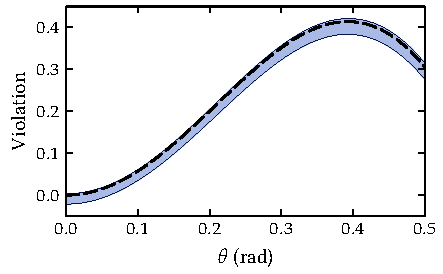
\includegraphics{figures_generated/bell/cooperative_N1.pdf}%
    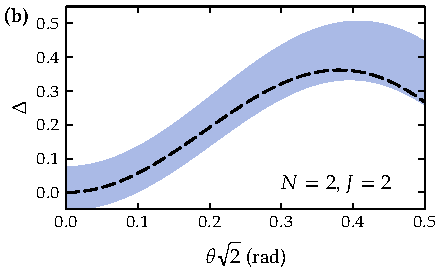
\includegraphics{figures_generated/bell/cooperative_N2.pdf}}

    \caption[Simulated Bell violation for cooperative states]{
    Simulated Bell violation $\Delta$ as a function of the relative polarizer angle $\theta$ for \textbf{(a)} one, and \textbf{(b)} two photon pairs using the positive-P distribution with \textbf{(a)} $2^{21}$ and \textbf{(b)} $2^{25}$ samples.
    The filled area corresponds to the estimated sampling error around the mean of $\Delta(\theta)$ for the sampled state, while the dashed line is the exact quantum mechanical prediction of this value.}%endcaption

    \label{fig:bell-ineq:cooperative:violation}
\end{figure}

Using the sampling method described in the previous subsection, we can now sample the positive-P distribution~\eqnref{bell-ineq:cooperative:pos-P} and calculate the violation~\eqnref{bell-ineq:cooperative:violation}.
We do that for the two-particle case $N=J=1$, and also for the four-particle case $N=J=2$, which has been observed experimentally~\cite{Howell2002}.
The results are plotted in~\figref{bell-ineq:cooperative:violation}, together with the analytical predictions~\eqnref{bell-ineq:cooperative:violation-1} and~\eqnref{bell-ineq:cooperative:violation-2}.
The second case requires significantly more samples to achieve a small enough sampling error, but it is clear that in both cases we were able to demonstrate the violation which is beyond the sampling error range.

% =============================================================================
\section{GHZM states}
\label{sec:bell-ineq:ghz}
% =============================================================================

We also perform mesoscopic Schr\"odinger cat state simulations, corresponding to recent ion-trap experiments with $M$ qubits.
These states violate a genuine multipartite Bell inequality, which means that it is impossible to confine the Bell violation to a microscopic part of the state.
Such inequalities require the measurement of all possible correlation functions at the highest order available.
We find two distinct scaling laws for the total computational difficulty, as measured by the number of samples required to obtain a given sampling error.

To understand the ultimate scaling properties of probabilistic sampling methods, we have also simulated higher order correlations that violate multipartite Bell inequalities.
These are found in quantum states that display Bell violations with $M$ observers, not just two.
The most well-known examples are the multimode entangled Greenberger-Horne-Zeilinger-Mermin (\abbrev{ghzm}) states~\cite{Greenberger1989,Mermin1990}, corresponding to ``Schr\"odinger Cat'' states.
Therefore, we considered \abbrev{ghzm} states, which describe $M$ spin-$\frac{1}{2}$ particles or qubits:
\begin{eqn}
\label{eqn:bell-ineq:ghz:state}
    \vert\Phi\rangle
    = \frac{1}{\sqrt{2}} \left(
        \ket{\uparrow\ldots\uparrow}
        + e^{i\phi} \ket{\downarrow\ldots\downarrow}
    \right).
\end{eqn}
Here $\ket{\uparrow}$ and $\ket{\downarrow}$ denote spin-up or spin-down particles in the $z$-direction.
As well as being of deep significance in quantum physics, such mesoscopic states have been generated in recent ion-trap experiments~\cite{Rowe2001,Leibfried2005,Monz2011}.

Quantum paradoxes are obtained on measuring an operator $\hat{A}$ which is defined as a linear combination of $2^{M}$ distinct $M$-th order correlation functions:
\begin{eqn}
\label{eqn:bell-ineq:ghz:operator}
    \hat{A}
    = \prod_{j=1}^{M} \left(
            \hat{\sigma}_j^x
            + i \hat{\sigma}_j^y
        \right),
\end{eqn}
where $s_j \in {-1, +1}$, and $\hat{\sigma}_j^x$ and $\hat{\sigma}_j^y$ are the Pauli spin operators acting on the $j$-th qubit.
We consider the constraints imposed by a \abbrev{lhv} on the expectation $A_{\lambda}(\phi) \equiv \langle \Phi(\phi) \vert \hat{A} \vert \Phi(\phi) \rangle_\lambda$ (where $\langle \rangle_{\lambda}$ stands for the expectation under \abbrev{lhv} assumptions) as compared to the predictions for these expectations given by quantum mechanics, $A_{\mathrm{QM}}(\phi) \equiv \langle \Phi(\phi) \vert \hat{A} \vert \Phi(\phi) \rangle$.

Mermin~\cite{Mermin1990} originally proved that for the phase difference $\phi=\pi/2$, \abbrev{qm} predicts that
\begin{eqn}
    \Imag A_{\mathrm{QM}}(\pi / 2)
    = 2^{M - 1},
\end{eqn}
while the \abbrev{lhv} bounds are
\begin{eqn2}
    \Imag A_{\lambda}(\pi / 2) & \le 2^{M/2},\quad & M\,\mathrm{is\,even}, \\
    \Imag A_{\lambda}(\pi / 2) & \le 2^{(M-1)/2},\quad & M\,\mathrm{is\,odd}.
\end{eqn2}
Ardehali~\cite{Ardehali1992} then proved that for $\phi=\pi$, the predictions are
\begin{eqn}
    -\Real A_{\mathrm{QM}}(\pi)
    = 2^{M - 1},
\end{eqn}
and
\begin{eqn2}
    -\Real A_{\lambda}(\pi) & \le 2^{(M-1)/2},\quad & M\,\mathrm{is\,even}, \\
    -\Real A_{\lambda}(\pi) & \le 2^{M/2},\quad & M\,\mathrm{is\,odd}.
\end{eqn2}
Here we transformed the original expressions given by Ardehali to the equivalent ones that use our definition of the target operator~\eqnref{bell-ineq:ghz:operator}.

It is clear that the Mermin inequalities are stronger for odd $M$, and the Ardehali ones are stronger for even $M$ (in particular, for $M = 2$ the Mermin inequalities are not even violated by \abbrev{qm}).
Therefore for our sampling tests in this section we will use the strongest of two inequalities, and the corresponding phase difference in the \abbrev{ghzm} state, for every $M$:
\begin{eqn2}
    F & = -\Real A_{\lambda}(\pi),\quad & M\,\mathrm{is\,even},\\
    F & = \Imag A_{\lambda}(\pi / 2),\quad & M\,\mathrm{is\,odd}.
\end{eqn2}
Consequently, for \abbrev{qm} and \abbrev{lhv} predictions we get the uniform \abbrev{qm} prediction $F_{\mathrm{QM}} = 2^{M - 1}$ and the inequality
\begin{eqn}
\label{eqn:bell-ineq:ghz:general-ineq}
    F_{\lambda} \le 2^{(M-1)/2}.
\end{eqn}
The relative violation can thus be made arbitrarily big to compensate for any imperfections in the measurements.


% =============================================================================
\subsection{Positive-P representation}
% =============================================================================

The na\"ive approach to the sampling of the state~\eqnref{bell-ineq:ghz:state} is to use the P-representation, same as we did in the previous section.
In general, spin-up and spin-down states are represented as $\ket{\uparrow}\equiv\ket{10}$ and $\ket{\downarrow}\equiv\ket{01}$, where $\ket{0}$ and $\ket{1}$ are number states, which allows for straightforward application of Pauli spin operators.

But for our particular choice of the target operator~\eqnref{bell-ineq:ghz:operator}, we can choose a simplified representation, which will halve the dimensionality of the resulting phase space: $\ket{\uparrow}\equiv\ket{0}$ and $\ket{\downarrow}\equiv\ket{1}$.
Since every term of $\hat{A}$ contains only one spin operator per qubit, it can be expressed in terms of creation and annihilation operators by replacing the spin operators with
\begin{eqn}
    \hat{\sigma}_j^x = \hat{a}_j + \hat{a}_j^\dagger,\quad
    \hat{\sigma}_j^y = \frac{1}{i} (\hat{a}_j - \hat{a}_j^\dagger),
\end{eqn}
from which the equivalent function of $\balpha$ and $\bbeta$ in P-representation immediately follows.

The P-representation of the target state is obtained with the canonical formula~\cite{Drummond1980}
\begin{eqn}
    P[\hat{\rho}]
    = \left( \frac{1}{4\pi^2} \right)^M
        \exp\left(
            -\frac{|\balpha -\bbeta^*|^2}{4}
        \right)
        \bra{\frac{1}{2} \left( \balpha + \bbeta^* \right)}
        \hat{\rho}
        \ket{\frac{1}{2} \left( \balpha + \bbeta^* \right)},
\end{eqn}
which for $\rho \equiv \ket{\Phi} \bra{\Phi}$ gives
\begin{eqn}
    P
    = \frac{1}{2 \pi^{2M}} e^{-|\bmu|^2} e^{-|\blambda^2|}
        \left|
            \prod_{j=1}^M \lambda_j + 1
        \right|^2,
\end{eqn}
where we have performed the variable change~\eqnref{bell-ineq:cooperative:mu-lambda}
\begin{eqn}
    \bmu = \frac{\balpha - \bbeta^*}{2},\quad
    \blambda = \frac{\balpha + \bbeta^*}{2}.
\end{eqn}

The sampling is performed using the rejection method with bounding $P$ as
\begin{eqn}
    P
    \le \frac{1}{2 \pi^{2M}} e^{-|\bmu|^2} e^{-|\blambda^2|}
        \left( \prod_{j=1}^M |\lambda_j|^2 + 1 \right).
\end{eqn}
Therefore, $P$ can be sampled using a combination of independent samples from Gaussian and gamma distributions, and then conditionally rejecting samples, as described in the previous section.

The phase space in this representation has $4M$ dimensions.
This can be further improved by using a specialized representation, allowing us to reduce the sampling error significantly, thus making the states with larger values of $M$ accessible for sampling.


% =============================================================================
\subsection{SU(2)-Q representation}
% =============================================================================

% acknowledgement
The theoretical derivation of the SU(2)-Q representation was performed by L.~E.~C.~Rosales-Z\'arate.
In this subsection we will briefly describe the framework of the representation, and apply it to our target state.

The positive-P representation does not impose any restrictions on the phase space, including the number states with population more than $1$ in the calculation of moments.
While it does not affect the calculated observable, it does increase the sampling error.
For the cases when we know that the system consists of binary states, more suitable representations exist.

We will consider a Q-representation~\cite{Husimi1940} for SU(2) coherent states~\cite{Arecchi1972,Zhang1990}:
\begin{eqn}
    \kket{\zvec}
    = \prod_{j=1}^{M} \left(
            \ket{\downarrow}_j + z_j \ket{\uparrow}_j
        \right),
\end{eqn}
where $z_j$ are complex numbers.
The SU(2)-Q function is the expectation value of the density operator over the SU(2) coherent states and is defined explicitly in a normalized form as:
\begin{eqn}
    Q[\hat{\rho}]
    = \left(
        \prod_{j=1}^M \frac{2}{\pi (1 + |z_j|^2)^3}
    \right) \bbra{\zvec} \hat{\rho} \kket{\zvec}.
\end{eqn}
For the target \abbrev{ghzm} state~\eqnref{bell-ineq:ghz:state}, the function takes the form of a probability distribution
\begin{eqn}
\label{eqn:bell-ineq:ghz:ghz-Q}
    Q
    = \frac{1}{2} \prod_{j=1}^M
        \frac{2}{\pi (1 + |z_j|^2)^3}
        \left|
            \prod_{j=1}^M z_j + e^{-i \phi}
        \right|^2
\end{eqn}

The sampling is again performed using the rejection method with bounding $Q$ as
\begin{eqn}
    Q
    \le \frac{1}{2} \prod_{j=1}^M
        \frac{2}{\pi (1 + |z_j|^2)^3}
        \left(
            \prod_{j=1}^M |z_j|^2 + 1
        \right),
\end{eqn}
and using the inverse sampling on both terms.
The expectation of $\hat{A}$ can be shown to be
\begin{eqn}
    A_{\mathrm{SU(2)-Q}}
    = \int
        6^M \prod_{j=1}^M \frac{z_j^*}{1 + |z_j|^2}
        Q(\zvec) \upd^2 \zvec.
\end{eqn}


% =============================================================================
\subsection{Results}
% =============================================================================

\begin{figure}
    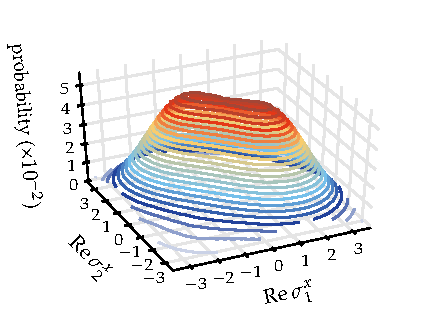
\includegraphics{figures_generated/bell/distribution_P1.pdf}%
    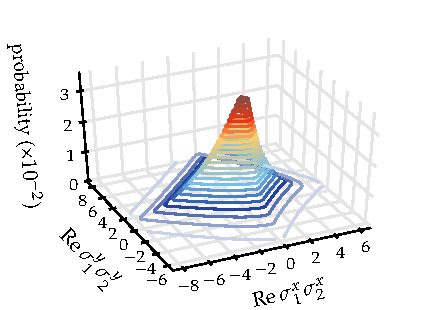
\includegraphics{figures_generated/bell/distribution_P2.pdf}\\
    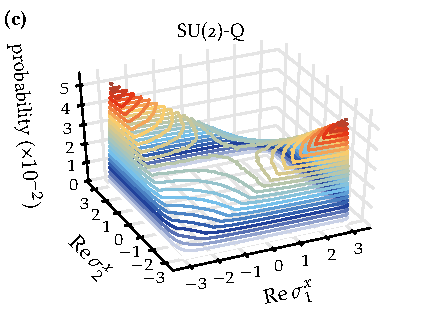
\includegraphics{figures_generated/bell/distribution_Q1.pdf}%
    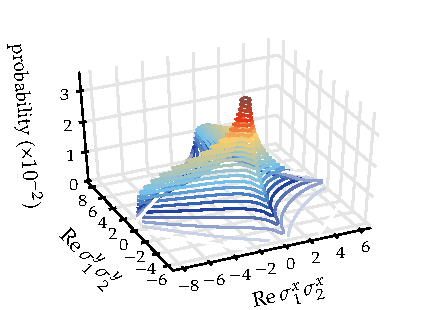
\includegraphics{figures_generated/bell/distribution_Q2.pdf}

    \caption[Correlations of first- and second-order moments in a Bell inequality]{
    Correlations for the different parts of the inequality~\eqnref{bell-ineq:ghz:general-ineq-M2}, in case of \textbf{(a, b)} positive-P and \textbf{(c, d)} SU(2)-Q representations, $10^8$ samples.}%endcaption

    \label{fig:bell-ineq:ghz:correlations}
\end{figure}

The difference between the positive-P and SU(2)-Q representations (and their difference from \abbrev{lhv} theories) can be illustrated on the inequality~\eqnref{bell-ineq:ghz:general-ineq} for $M = 2$:
\begin{eqn}
\label{eqn:bell-ineq:ghz:general-ineq-M2}
    - \langle \hat{\sigma}_1^x \hat{\sigma}_2^x \rangle_{\lambda}
    + \langle \hat{\sigma}_1^y \hat{\sigma}_2^y \rangle_{\lambda}
    \le \sqrt{2}.
\end{eqn}
The real parts of the correlations in this expression for both representations used are plotted in~\figref{bell-ineq:ghz:correlations}.

The main feature of quasiprobability representations is apparent: neither of them limits the value of $\Real \sigma_1^x$ or $\Real \sigma_2^x$ to the range $[-1, 1]$ as would happen in a \abbrev{lhv} theory.
This means that the Bell theorem does not apply to these results because the sampled values differ from their physical equivalents.
Moreover, the plots for the SU(2)-Q show that in this representation the correlations are more peaked, and also do not have exponential tails as the ones in the positive-P representation.
This, in addition to the reduced phase space dimensionality, allows the sampling with SU(2)-Q representation for high values of $M$.

\begin{figure}
    \centerline{%
    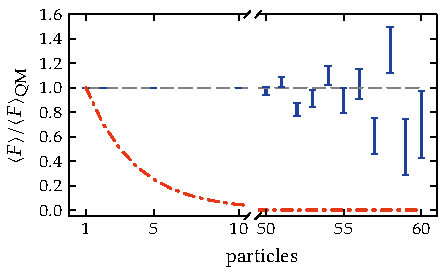
\includegraphics{figures_generated/bell/ghz_violations.pdf}%
    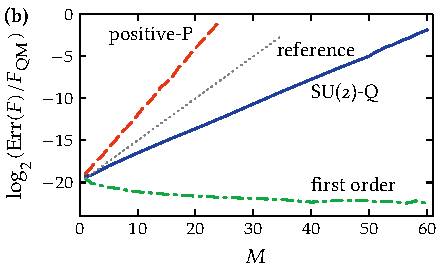
\includegraphics{figures_generated/bell/ghz_errors.pdf}}

    \caption[Violation of Bell inequality in \abbrev{ghzm} states]{
    Violations of the inequality~\eqnref{bell-ineq:ghz:general-ineq} for multi-particle \abbrev{ghzm} states.
    \textbf{(a)} Blue bars show the expectation $F$ simulated using the SU(2)-Q representation, with the length of the bars corresponding to the sampling error.
    The values of expectations and errors are normalized by the quantum mechanical prediction for the corresponding $M$.
    The horizontal grey dashed line gives the quantum prediction.
    The red dash-dotted line is the \abbrev{lhv} prediction, which gives a Bell violation when the expectation $F$ is above this line.
    \textbf{(b)} Relative sampling errors for $F$ simulated using the positive-P (red dashed line) and SU(2)-Q (blue solid line) representations.
    Sampling errors for a first order correlation (total number of ``spin-ups'') in the SU(2)-Q representation are plotted as a green dashed line.
    The grey dotted reference line $\log_2 \mathrm{error} \propto M / 2$ shows the point at which the sampling errors would give scaling properties as slow as an experimental measurement.}%endcaption

    \label{fig:bell-ineq:ghz:violation}
\end{figure}

The results of such sampling are shown in~\figref{bell-ineq:ghz:violation}.
We used seven nVidia Tesla M2090 \abbrev{gpu}s to generate $10^{12}$ samples of the distribution~\eqnref{bell-ineq:ghz:ghz-Q} and calculate the required correlation for the values of $M$ up to $60$, and these samples were used to test the inequality~\eqnref{bell-ineq:ghz:general-ineq}.
This corresponds to measurement of $10^{18}$ distinct sixtieth order correlation functions.
As~\figref{bell-ineq:ghz:violation},~(a) demonstrates, Bell violations were verified in all cases, although closer to $M=60$ the sampling error grew almost enough to invalidate the results.
Larger values of $M$ would require more samples.

We also investigated the growth of sampling errors for $F$ with the positive-P and SU(2)-Q representations, as shown in~\figref{bell-ineq:ghz:violation},~(b).
In order to have some reference for comparisons, we also plotted the sampling error for the total number of ``spin-ups''
\begin{eqn}
    N = \langle\sum_{j=1}^M (\hat{\sigma}_j^z + 1 )/2 \rangle.
\end{eqn}
This low-order spin correlation requires a linearly growing amount of measurements in the experiment as compared to the exponentially growing amount for $F$.
As the plot shows, the sampling error for $N$ even slowly decreases as $M$ grows.
This explains why low-order correlations could be efficiently sampled in previous work, for much larger Hilbert spaces than the ones studied here.

On the other hand, high-order correlations showed exponentially growing sampling error.
In case of positive-P the relative error scales as $2^{4M/5}$, which with the chosen number of samples, produces Bell violations only up to $M=25$.
The SU(2)-Q representation shows much better results with the relative error scaling as $2^{M/3}$, so the time taken by the simulation at constant error scales as $2^{2M/3}$.
An experiment measuring the same quantity would take time proportional to $2^M$ since it would have to perform measurements for exponentially many settings.
Thus, the probabilistic sampling of the SU(2)-Q function scales better than experiment for high-order correlations.

These results show that probabilistic sampling is a perfectly viable technique both for low- and high-order correlations.
Low-order correlations are the ones most commonly measured, and sampling errors in these are insensitive to scaling up to mesoscopic sizes.
Correlations of the same order as the system size are still exponentially hard, but a carefully chosen quasiprobability representation can give an exponential advantage over experimental scaling.

% =============================================================================
\section{Conclusion}
% =============================================================================

